\documentclass[
]{jss}

\usepackage[utf8]{inputenc}

\providecommand{\tightlist}{%
  \setlength{\itemsep}{0pt}\setlength{\parskip}{0pt}}

\author{
Hanne Oberman\\Utrecht University \And Johanna Munoz Avila\\University
Medical Center Utrecht \And Valentijn\\University Medical Center Utrecht
\AND Gerko Vink\\Utrecht University \And Thomas Debray\\University
Medical Center Utrecht
}
\title{Imputation of Incomplete Multilevel Data with \pkg{mice}}

\Plainauthor{Hanne Oberman, Johanna Munoz Avila, Valentijn, Gerko
Vink, Thomas Debray}
\Plaintitle{Imputation of Incomplete Multilevel Data with mice}
\Shorttitle{\pkg{mice}: Multilevel}


\Abstract{
Tutorial paper on imputing incomplete multilevel data with \pkg{mice}.
Including methods for ignorable and non-ignorable missingness. AKA
missing on so many levels.
}

\Keywords{missing data, multilevel, clustering, \proglang{R}}
\Plainkeywords{missing data, multilevel, clustering, R}

%% publication information
%% \Volume{50}
%% \Issue{9}
%% \Month{June}
%% \Year{2012}
%% \Submitdate{}
%% \Acceptdate{2012-06-04}

\Address{
    Hanne Oberman\\
    Utrecht University\\
    Padualaan 14\\
3584 CH Utrecht\\
  E-mail: \email{h.i.oberman@uu.nl}\\
  URL: \url{https://hanneoberman.github.io/}\\~\\
          }

% Pandoc syntax highlighting

% Pandoc citation processing


\usepackage{amsmath}

\begin{document}

\hypertarget{introduction}{%
\section{Introduction}\label{introduction}}

\hypertarget{multilevel-data}{%
\subsection{Multilevel data}\label{multilevel-data}}

\begin{itemize}
\item
  What is clustering/multilevel data? In this paper, we discuss grouped
  observations, not longitudinal data (within-patient clustering). What
  do we mean by clustering? In the medical field: Clustering by studies
  (IPDMA), hospitals in registries, multi-center studies etc. In other
  fields: e.g.~official stats clustering at country-level, or social
  sciences clustering at school-level (related to the sampling design).
\item
  What is heterogeniety (i.e.~variability within studies vs.~variability
  between studies)? ADD: Figure to show difference between patient-level
  datapoints vs cluster-level datapoints. And different data frame
  formats.
\item
  What methods are required to analyze multilevel data? Random effects
  for intercept term, predictor effects, and/or variance residual error.
  Add references, e.g. \citet{hox17}.
\end{itemize}

\hypertarget{missing-data}{%
\subsection{Missing data}\label{missing-data}}

\begin{itemize}
\item
  Why/where does missingness occur? I.e., not only patient-level but
  also cluster-level.
\item
  How can we categorize this? Systematic vs sporadic missingness, see
  \citet{resc13}. ADD: visualization of systematic vs sporadic
  missingness. Within systematic we have always missing (same value per
  cluster) and non-measured variables (may differ per patient). TODO:
  adjust md pattern to match text.
\end{itemize}

\begin{CodeChunk}


\begin{center}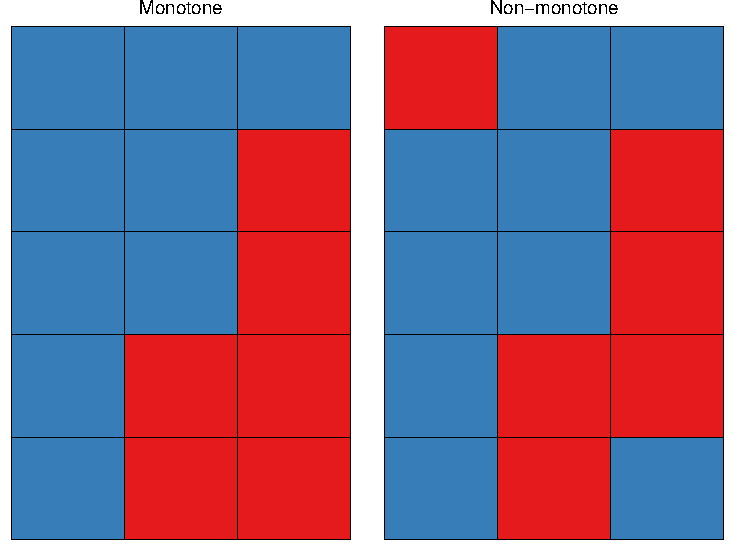
\includegraphics{Multilevel-Missing-Data_files/figure-latex/patterns-1} \end{center}

\end{CodeChunk}

\begin{itemize}
\item
  Why are standard (ad hoc) missing data methods not well suited?
\item
  What other methods are available? General overview of approaches, see
  \citet{audi18} \citet{grun18}. E.g., imputation of study level versus
  patient-level covariates, and one-stage imputation versus two-stage
  imputation methods.
\item
  Additional problem addressed in this paper: handling MNAR.
\end{itemize}

\hypertarget{aim-of-this-paper}{%
\subsection{Aim of this paper}\label{aim-of-this-paper}}

\begin{itemize}
\item
  Provide practical guidelines with code snippets for imputation of
  incomplete multilevel data.
\item
  Case study options: metamisc::impact (IPD), GREAT (IPD).
\end{itemize}

\hypertarget{workflows}{%
\section{Workflows}\label{workflows}}

\hypertarget{modeling-choices}{%
\subsection{Modeling choices}\label{modeling-choices}}

\begin{itemize}
\item
  ADD: Section with more in-depth info on different data types and
  suitable methods. Add some equations, but not too much -\textgreater{}
  grow in complexity.
\item
  Ideally we impute with random everything and heteroscedastic errors:
  most generic method (no worry about congeneiality) --\textgreater{}
  explain predictor matrix. Just mention that we should think about
  random intercept/slope, but just refer to other papers. This paper is
  just a software tutorial. --\textgreater{} Typically, at least random
  intercepts, but often random slopes as well. Refer to other papers for
  background, we'll focus just on the software implementation of the
  situations mentioned there. Sometimes there's little reason to assume
  some variable is affected by heterogeniety. We won't focus on
  congeneiality, that's too complex for 2-3 papers.
\end{itemize}

\hypertarget{conditional-models}{%
\subsection{Conditional models}\label{conditional-models}}

\begin{itemize}
\item
  How to define the imputation model(s) in mice?
\item
  What do the different implementations look like?
\end{itemize}

\hypertarget{pooling}{%
\subsection{Pooling}\label{pooling}}

\begin{itemize}
\item
  Pooling `regular' parameters vs more `exotic' parameters (SE of
  residual errors, or autocorreletion)
\item
  ADD: export mids objects to other packages like lme4 or coxme(?)
\end{itemize}

\hypertarget{think-about-adding}{%
\section{Think about adding}\label{think-about-adding}}

\begin{itemize}
\item
  JOMO in mice --\textgreater{} on the side for now
\item
  Additional levels of clustering
\end{itemize}

\renewcommand\refname{References}
\bibliography{../References/multilevelmice.bib}


\end{document}
